\section{Lattice Visualization} \label{appendix:lattice-visualisation}

\begin{minipage}{\linewidth}
    \centering
    \makebox[\textwidth][c]{
        \makebox[1.25\textwidth][c]{
            \makebox[0.40\textwidth][l]{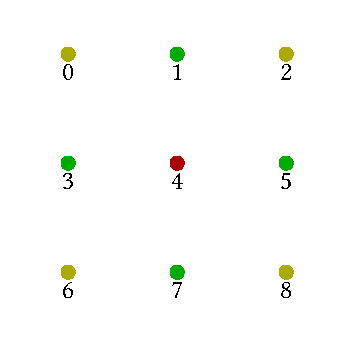
\includegraphics[width=0.33\textwidth]{./../appendix/lattice_visualization/square,size=2,np.pdf}}
            \makebox[0.40\textwidth][l]{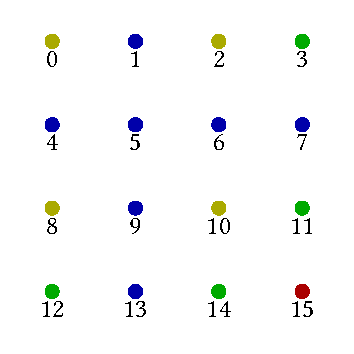
\includegraphics[width=0.33\textwidth]{./../appendix/lattice_visualization/square,size=3,p.pdf}}
            \makebox[0.40\textwidth][l]{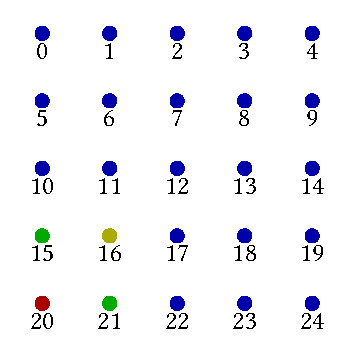
\includegraphics[width=0.33\textwidth]{./../appendix/lattice_visualization/square,size=4,np.pdf}}
        }
    }

    \captionof{figure}{A visualization of the \textbf{2D-square} lattice structure, measured in this thesis. 
        The lattices from left to right can be described by the parameters\\
        1: \emph{size=2, non-periodic}\,\,\,\, 2: \emph{size=3, periodic}\,\,\,\, 3: \emph{size=4, non-periodic}
    }
    \label{fig:appendix-square-lattices}
\end{minipage}

\vspace{0.5cm}

\begin{minipage}{\linewidth}
    \centering
    \makebox[\textwidth][c]{
        \makebox[1.25\textwidth][c]{
            \makebox[0.40\textwidth][l]{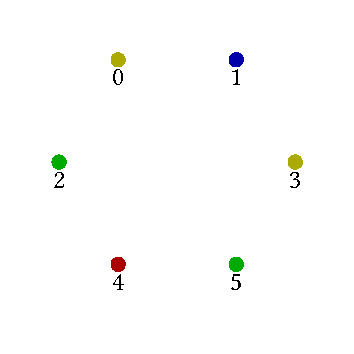
\includegraphics[width=0.33\textwidth]{./../appendix/lattice_visualization/hexagonal,size=1,np.pdf}}
            \makebox[0.40\textwidth][l]{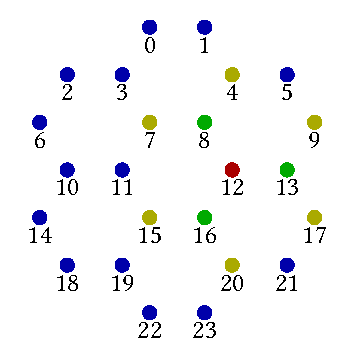
\includegraphics[width=0.33\textwidth]{./../appendix/lattice_visualization/hexagonal,size=2,np.pdf}}
            \makebox[0.40\textwidth][l]{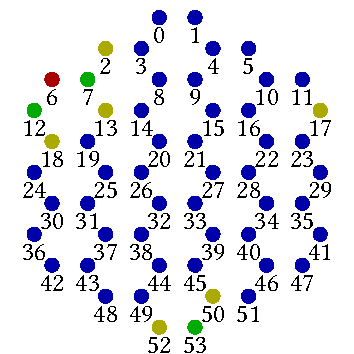
\includegraphics[width=0.33\textwidth]{./../appendix/lattice_visualization/hexagonal,size=3,p.pdf}}
        }
    }

    \vspace{0.3cm}
    \captionof{figure}{A visualization of the \textbf{2D-hexagonal} lattice structure, measured in this thesis. 
        The lattices from left to right can be described by the parameters \\
        1: \emph{size=1, non-periodic}\,\,\,\, 2: \emph{size=2, non-periodic}\,\,\,\, 3: \emph{size=3, periodic}
    }
    \label{fig:appendix-hexagonal-lattices}
\end{minipage}

\vspace{0.4cm}

\begin{minipage}{\linewidth}
    \centering
    \makebox[\textwidth][c]{
        \makebox[1.25\textwidth][c]{
            \makebox[0.40\textwidth][l]{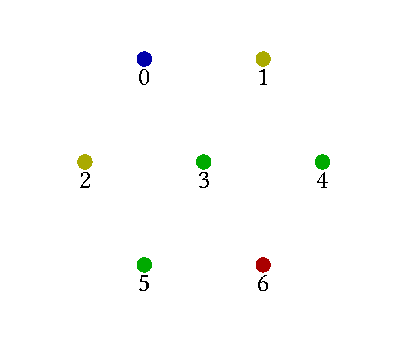
\includegraphics[width=0.33\textwidth]{./../appendix/lattice_visualization/trigonal_hexagonal,size=1,np.pdf}}
            \makebox[0.40\textwidth][l]{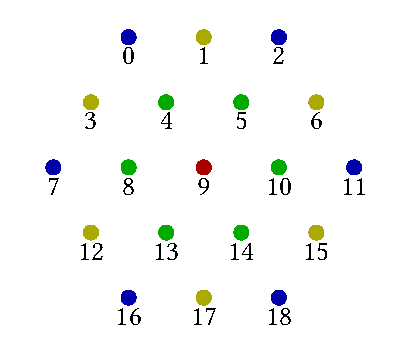
\includegraphics[width=0.33\textwidth]{./../appendix/lattice_visualization/trigonal_hexagonal,size=2,np.pdf}}
            \makebox[0.40\textwidth][l]{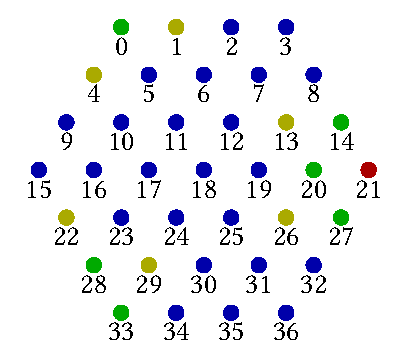
\includegraphics[width=0.33\textwidth]{./../appendix/lattice_visualization/trigonal_hexagonal,size=3,p.pdf}}
        }
    }
    
    \vspace{0.5cm}
    \captionof{figure}{A visualization of the \textbf{2D-trigonal\_hexagonal} lattice structure, measured in this thesis. 
        The lattices from left to right can be described by the parameters \\
        1: \emph{size=1, non-periodic}\,\,\,\, 2: \emph{size=2, non-periodic}\,\,\,\, 3: \emph{size=3, periodic}
    }
    \label{fig:appendix-trigonal_hexagonal-lattices}
\end{minipage}

% HERE SHOULD THE PAGE-BREAK BE. i love latex, but stuff like this infuriates me to get correct
\newpage
\makebox{\vspace{5cm}}\\

\begin{minipage}{\linewidth}
    \centering
    \makebox[\textwidth][c]{
        \makebox[1.25\textwidth][c]{
            \makebox[0.40\textwidth][l]{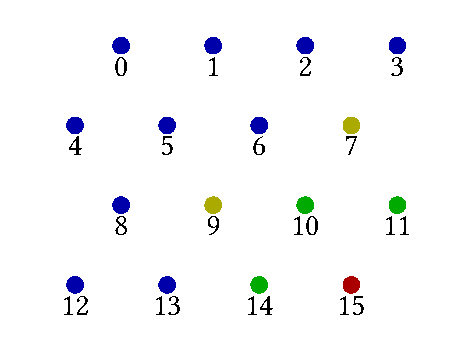
\includegraphics[width=0.33\textwidth]{./../appendix/lattice_visualization/trigonal_square,size=2,np.pdf}}
            \makebox[0.40\textwidth][l]{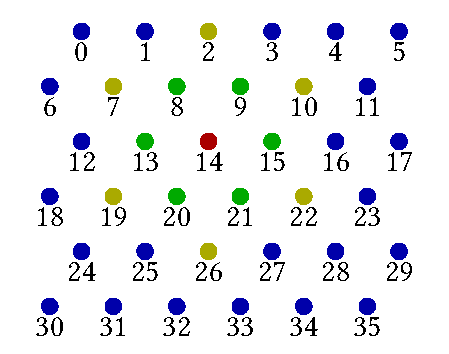
\includegraphics[width=0.33\textwidth]{./../appendix/lattice_visualization/trigonal_square,size=3,np.pdf}}
            \makebox[0.40\textwidth][l]{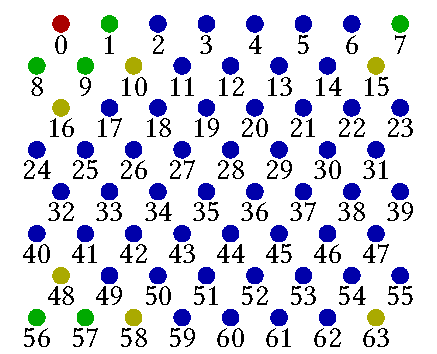
\includegraphics[width=0.33\textwidth]{./../appendix/lattice_visualization/trigonal_square,size=4,p.pdf}}
        }
    }

    \vspace{0.4cm}
    \captionof{figure}{A visualization of the \textbf{2D-trigonal\_square} lattice structure, measured in this thesis. 
        The lattices from left to right can be described by the parameters \\
        1: \emph{size=2, non-periodic}\,\,\,\, 2: \emph{size=3, non-periodic}\,\,\,\, 3: \emph{size=4, periodic}
    }
    \label{fig:appendix-trigonal_square-lattices}
\end{minipage}

\vspace{1.2cm}

\begin{minipage}{\linewidth}
    \centering
    \makebox[\textwidth][c]{
        \makebox[1.25\textwidth][c]{
            \makebox[0.40\textwidth][c]{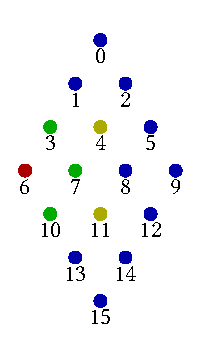
\includegraphics[width=0.20\textwidth]{./../appendix/lattice_visualization/trigonal_diamond,size=3,np.pdf}}
            \makebox[0.40\textwidth][c]{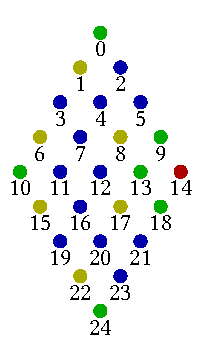
\includegraphics[width=0.20\textwidth]{./../appendix/lattice_visualization/trigonal_diamond,size=4,p.pdf}}
            \makebox[0.40\textwidth][c]{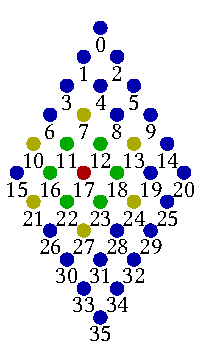
\includegraphics[width=0.20\textwidth]{./../appendix/lattice_visualization/trigonal_diamond,size=5,np.pdf}}
        }
    }

    \vspace{0.4cm}
    \captionof{figure}{A visualization of the \textbf{2D-trigonal\_diamond} lattice structure, measured in this thesis. 
        The lattices from left to right can be described by the parameters \\
        1: \emph{size=3, non-periodic}\,\,\,\, 2: \emph{size=4, periodic}\,\,\,\, 3: \emph{size=5, non-periodic}
    }
    \label{fig:appendix-trigonal_diamond-lattices}
\end{minipage}

\vspace{1.2cm}

\begin{minipage}{\linewidth}
    \centering
    \makebox[\textwidth][c]{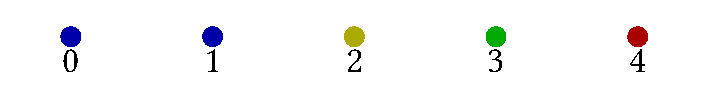
\includegraphics[width=0.80\textwidth]{./../appendix/lattice_visualization/linear,size=5,np.pdf}}
    \vspace*{0.2cm}
    \makebox[\textwidth][c]{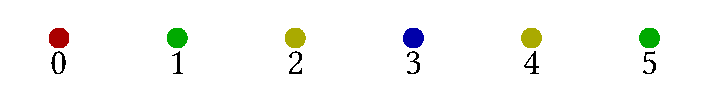
\includegraphics[width=0.80\textwidth]{./../appendix/lattice_visualization/linear,size=6,p.pdf}}
    \vspace*{0.2cm}
    \makebox[\textwidth][c]{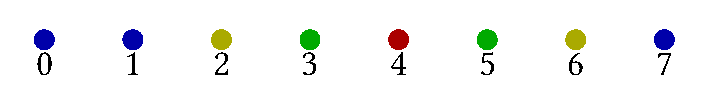
\includegraphics[width=0.80\textwidth]{./../appendix/lattice_visualization/linear,size=8,np.pdf}}

    \vspace{0.2cm}
    \captionof{figure}{A visualization of the \textbf{1D-linear} lattice structure, measured in this thesis. 
        The lattices from top to bottom can be described by the parameters \\
        1: \emph{size=5, non-periodic}\,\,\,\, 2: \emph{size=6, periodic}\,\,\,\, 3: \emph{size=8, non-periodic}
    }
    \label{fig:appendix-linear-lattices}
\end{minipage}

\newpage